\chapter{Project description}
\textit{This chapter seeks to explain the design and implementation of the project along with the tests used for improving the system.}
\section{Architecture}
The system consist of the CDU and a number of sensor nodes. This is seen on figure \ref{fig:systembdd}. Every sensor is powered by the custom power line communication bus. All communication is transmitted via the same bus. 
\begin{figure}[H]
	\centering
	\includegraphics[width=.9\textwidth]{billeder/11ProjectDescription/systembdd}
	\caption{System overview}
	\label{fig:systembdd}
\end{figure}
The bus is the central part of this chapter. It consists of several layers as displayed on figure \ref{fig:systemlayers}. The design of the protocol layer is found in the architecture document. The design of the subsequent layers can be found in the design and implementation document.
\begin{figure}[H]
	\centering
	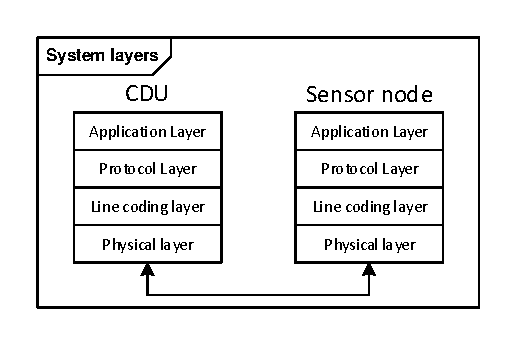
\includegraphics[width=.6\textwidth]{billeder/11ProjectDescription/System_Layers}
	\caption{System Layers}
	\label{fig:systemlayers}
\end{figure}
The protocol was designed with respects to already known protocols such as Modbus and I$^{2}$C. The principle of a start code and addressing was inspired by I$^{2}$C while the idea of function codes was inspired by Modbus. A data length multiplier tells the receiver how many bytes of data that are in the full message. A CRC check in the end ensures that the message was received correctly. This is further explained by table \ref{table:stdmsgtosensor}.
\begin{table}[H]
\centering
\begin{tabular}{|l|l|l|l|l|l|}
	\hline
	Start Sequence & Address & Function Code & DLM & Data & CRC  \\ \hline
	1 nibble & 1 nibble	& 1 nibble & 1 nibble & n bytes & 1 byte\\
	\hline
\end{tabular}
\caption{Message format for writing and reading}
\label{table:stdmsgtosensor}
\end{table}
\section{Design and implementation}

\section{Tests}
